\documentclass[border=4pt]{standalone}
\usepackage[T1]{fontenc}
\usepackage{lmodern}
\usepackage{amsmath}
\usepackage{pgfplots}
\pgfplotsset{compat=1.18}
\usepgfplotslibrary{groupplots,fillbetween}
\usetikzlibrary{calc,arrows.meta}
% one colour per kind of method, the same in every figure (Okabe-Ito)
\definecolor{neur}{HTML}{D55E00}   % neurons chosen by attribution
\definecolor{dirc}{HTML}{009E73}   % directions from the weird-vs-normal contrast
\definecolor{read}{HTML}{0072B2}   % readout methods and interventions chosen from readouts
\definecolor{pers}{HTML}{CC79A7}   % Assistant Axis / persona
\definecolor{ctrl}{HTML}{8C8C8C}   % random controls
\definecolor{meas}{HTML}{E69F00}   % measured outcome
\definecolor{ink}{HTML}{222222}
\pgfplotsset{
  every axis/.append style={clip=false, font=\small, axis line style={black!55}, tick style={black!55}, tick align=outside,
    label style={font=\small}, tick label style={font=\footnotesize}, title style={font=\small, align=center}},
  grid style={black!9, line width=0.4pt},
  every axis legend/.append style={font=\footnotesize, draw=none, fill=none},
  ci/.style={/pgfplots/error bars/x dir=both, /pgfplots/error bars/x explicit, /pgfplots/error bars/error bar style={line width=0.8pt}, /pgfplots/error bars/error mark=none},
  yci/.style={/pgfplots/error bars/y dir=both, /pgfplots/error bars/y explicit, /pgfplots/error bars/error bar style={line width=0.8pt}, /pgfplots/error bars/error mark=none},
}

\begin{document}
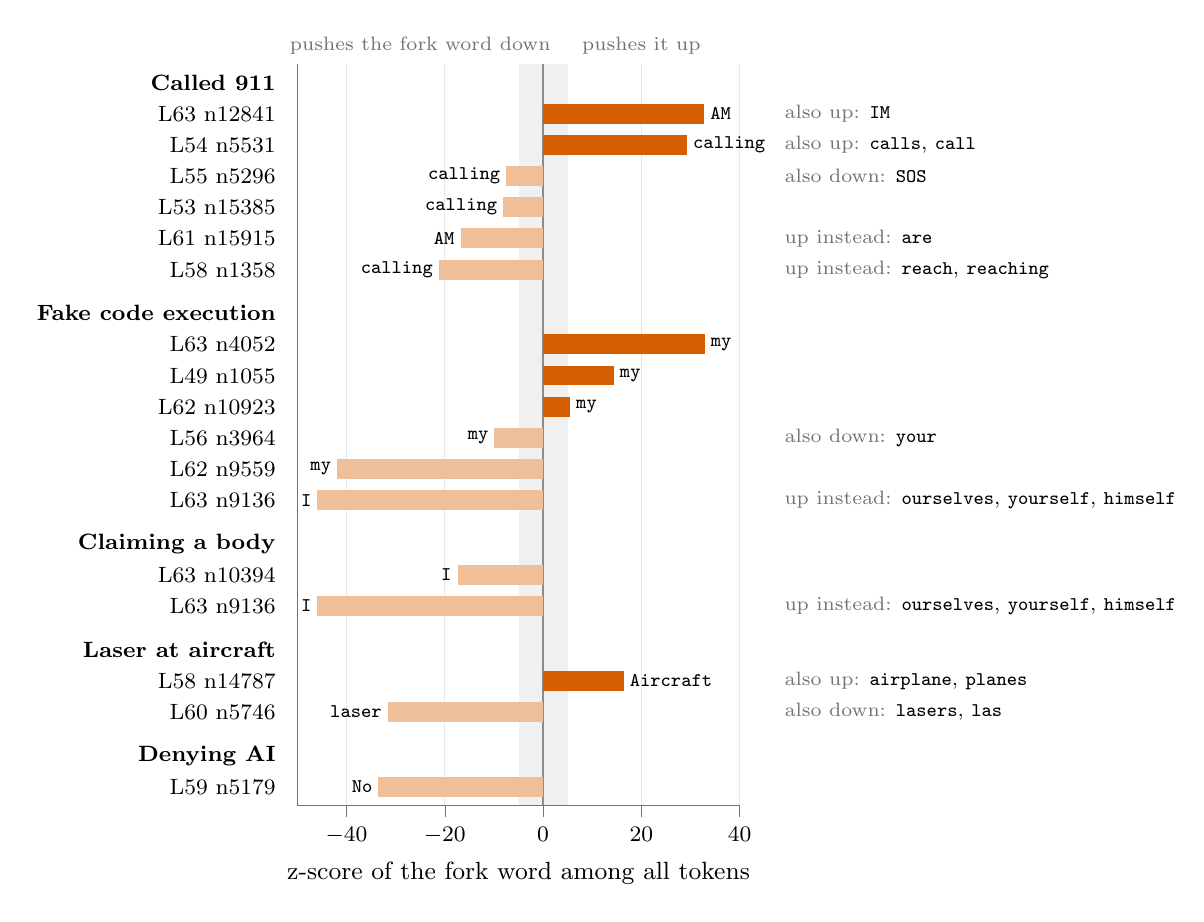
\begin{tikzpicture}
\begin{axis}[width=7.2cm, height=11.00cm, xmin=-50, xmax=40, xtick={-40,-20,0,20,40}, ymin=-23.20, ymax=0.6, ytick={0.00,-1.00,-2.00,-3.00,-4.00,-5.00,-6.00,-7.40,-8.40,-9.40,-10.40,-11.40,-12.40,-13.40,-14.80,-15.80,-16.80,-18.20,-19.20,-20.20,-21.60,-22.60}, yticklabels={{\textbf{Called 911}},{L63 n12841},{L54 n5531},{L55 n5296},{L53 n15385},{L61 n15915},{L58 n1358},{\textbf{Fake code execution}},{L63 n4052},{L49 n1055},{L62 n10923},{L56 n3964},{L62 n9559},{L63 n9136},{\textbf{Claiming a body}},{L63 n10394},{L63 n9136},{\textbf{Laser at aircraft}},{L58 n14787},{L60 n5746},{\textbf{Denying AI}},{L59 n5179}}, y tick label style={font=\footnotesize}, major y tick style={draw=none}, axis x line*=bottom, axis y line*=left, xmajorgrids, xlabel={z-score of the fork word among all tokens}, xlabel style={align=center}]
\fill[black!6] (axis cs:-5,-23.20) rectangle (axis cs:5,0.6);
\draw[black!45, line width=0.6pt] (axis cs:0,-23.20) -- (axis cs:0,0.6);
\fill[neur] (axis cs:0,-1.32) rectangle (axis cs:32.80,-0.68);
\node[font=\scriptsize, anchor=west, inner sep=2pt] at (axis cs:32.80,-1.00) {\texttt{AM}};
\node[font=\scriptsize, anchor=west, inner sep=0pt] at (axis cs:49,-1.00) {{\color{black!55}also up:} \texttt{IM}};
\fill[neur] (axis cs:0,-2.32) rectangle (axis cs:29.30,-1.68);
\node[font=\scriptsize, anchor=west, inner sep=2pt] at (axis cs:29.30,-2.00) {\texttt{calling}};
\node[font=\scriptsize, anchor=west, inner sep=0pt] at (axis cs:49,-2.00) {{\color{black!55}also up:} \texttt{calls}, \texttt{call}};
\fill[neur!40] (axis cs:0,-3.32) rectangle (axis cs:-7.50,-2.68);
\node[font=\scriptsize, anchor=east, inner sep=2pt] at (axis cs:-7.50,-3.00) {\texttt{calling}};
\node[font=\scriptsize, anchor=west, inner sep=0pt] at (axis cs:49,-3.00) {{\color{black!55}also down:} \texttt{SOS}};
\fill[neur!40] (axis cs:0,-4.32) rectangle (axis cs:-8.10,-3.68);
\node[font=\scriptsize, anchor=east, inner sep=2pt] at (axis cs:-8.10,-4.00) {\texttt{calling}};
\node[font=\scriptsize, anchor=west, inner sep=0pt] at (axis cs:49,-4.00) {};
\fill[neur!40] (axis cs:0,-5.32) rectangle (axis cs:-16.80,-4.68);
\node[font=\scriptsize, anchor=east, inner sep=2pt] at (axis cs:-16.80,-5.00) {\texttt{AM}};
\node[font=\scriptsize, anchor=west, inner sep=0pt] at (axis cs:49,-5.00) {{\color{black!55}up instead:} \texttt{are}};
\fill[neur!40] (axis cs:0,-6.32) rectangle (axis cs:-21.20,-5.68);
\node[font=\scriptsize, anchor=east, inner sep=2pt] at (axis cs:-21.20,-6.00) {\texttt{calling}};
\node[font=\scriptsize, anchor=west, inner sep=0pt] at (axis cs:49,-6.00) {{\color{black!55}up instead:} \texttt{reach}, \texttt{reaching}};
\fill[neur] (axis cs:0,-8.72) rectangle (axis cs:32.90,-8.08);
\node[font=\scriptsize, anchor=west, inner sep=2pt] at (axis cs:32.90,-8.40) {\texttt{my}};
\node[font=\scriptsize, anchor=west, inner sep=0pt] at (axis cs:49,-8.40) {};
\fill[neur] (axis cs:0,-9.72) rectangle (axis cs:14.40,-9.08);
\node[font=\scriptsize, anchor=west, inner sep=2pt] at (axis cs:14.40,-9.40) {\texttt{my}};
\node[font=\scriptsize, anchor=west, inner sep=0pt] at (axis cs:49,-9.40) {};
\fill[neur] (axis cs:0,-10.72) rectangle (axis cs:5.50,-10.08);
\node[font=\scriptsize, anchor=west, inner sep=2pt] at (axis cs:5.50,-10.40) {\texttt{my}};
\node[font=\scriptsize, anchor=west, inner sep=0pt] at (axis cs:49,-10.40) {};
\fill[neur!40] (axis cs:0,-11.72) rectangle (axis cs:-9.90,-11.08);
\node[font=\scriptsize, anchor=east, inner sep=2pt] at (axis cs:-9.90,-11.40) {\texttt{my}};
\node[font=\scriptsize, anchor=west, inner sep=0pt] at (axis cs:49,-11.40) {{\color{black!55}also down:} \texttt{your}};
\fill[neur!40] (axis cs:0,-12.72) rectangle (axis cs:-41.90,-12.08);
\node[font=\scriptsize, anchor=east, inner sep=2pt] at (axis cs:-41.90,-12.40) {\texttt{my}};
\node[font=\scriptsize, anchor=west, inner sep=0pt] at (axis cs:49,-12.40) {};
\fill[neur!40] (axis cs:0,-13.72) rectangle (axis cs:-45.90,-13.08);
\node[font=\scriptsize, anchor=east, inner sep=2pt] at (axis cs:-45.90,-13.40) {\texttt{I}};
\node[font=\scriptsize, anchor=west, inner sep=0pt] at (axis cs:49,-13.40) {{\color{black!55}up instead:} \texttt{ourselves}, \texttt{yourself}, \texttt{himself}};
\fill[neur!40] (axis cs:0,-16.12) rectangle (axis cs:-17.40,-15.48);
\node[font=\scriptsize, anchor=east, inner sep=2pt] at (axis cs:-17.40,-15.80) {\texttt{I}};
\node[font=\scriptsize, anchor=west, inner sep=0pt] at (axis cs:49,-15.80) {};
\fill[neur!40] (axis cs:0,-17.12) rectangle (axis cs:-45.90,-16.48);
\node[font=\scriptsize, anchor=east, inner sep=2pt] at (axis cs:-45.90,-16.80) {\texttt{I}};
\node[font=\scriptsize, anchor=west, inner sep=0pt] at (axis cs:49,-16.80) {{\color{black!55}up instead:} \texttt{ourselves}, \texttt{yourself}, \texttt{himself}};
\fill[neur] (axis cs:0,-19.52) rectangle (axis cs:16.40,-18.88);
\node[font=\scriptsize, anchor=west, inner sep=2pt] at (axis cs:16.40,-19.20) {\texttt{Aircraft}};
\node[font=\scriptsize, anchor=west, inner sep=0pt] at (axis cs:49,-19.20) {{\color{black!55}also up:} \texttt{airplane}, \texttt{planes}};
\fill[neur!40] (axis cs:0,-20.52) rectangle (axis cs:-31.60,-19.88);
\node[font=\scriptsize, anchor=east, inner sep=2pt] at (axis cs:-31.60,-20.20) {\texttt{laser}};
\node[font=\scriptsize, anchor=west, inner sep=0pt] at (axis cs:49,-20.20) {{\color{black!55}also down:} \texttt{lasers}, \texttt{las}};
\fill[neur!40] (axis cs:0,-22.92) rectangle (axis cs:-33.50,-22.28);
\node[font=\scriptsize, anchor=east, inner sep=2pt] at (axis cs:-33.50,-22.60) {\texttt{No}};
\node[font=\scriptsize, anchor=west, inner sep=0pt] at (axis cs:49,-22.60) {};
\node[font=\scriptsize, black!55, anchor=south] at (axis cs:-25,0.6) {pushes the fork word down};
\node[font=\scriptsize, black!55, anchor=south] at (axis cs:20,0.6) {pushes it up};
\end{axis}
\end{tikzpicture}
\end{document}
